\documentclass{article}
\usepackage{tikz}


\title{Engineering Physics I}
\author{Conrad A. Mearns}

\begin{document}

\maketitle

\noindent
\Large
Significant Figures\\
\normalsize
\noindent
When multiplying or dividing, the result is as precise as the least precise input to the number of digits.\\
Example: $54.3 * 6.8991 = 374.62113$, truncated to $374$ or rounded to $375$.\\\\

\noindent
When adding or subtracting, the result is as precise as the least precise input to the nuber of digits post decimal place.\\
Example: $10.65 + 3.0 = 13.65$, truncated to $13.6$ or rounded to $13.7$.\\\\

\noindent
As a general rule (from the professor), round up down to the nearset even number, as always rounding up will accumulate more error.

\noindent
\Large
Variables of Movement and Position\\
\normalsize

\begin{enumerate}
  \item Position: Location in space with respect to another object or coordinate system.\\
    $x, y, z$
  \item Displacement: Difference in position at two different times.\\
    $\Delta x, \Delta y, \Delta z, \Delta x = x_2 - X_1$
  \item Average Velocity: Displacement divided by time.\\\
    $v_{avg}, v_{avg} = \frac{\Delta x}{\Delta t}$
  \item Speed: Total distance divided by time.\\
    $s, s \equiv \frac{d}{t}$
  \item Instantanious Velocity: Velocity measured at a single time.\\
    $v, v = \lim_{t \to a}\frac{\Delta x}{\Delta t} = \lim_{t \to a}\frac{x_2 - x_1}{t_2 - t_1}$
\end{enumerate}

\noindent
\Large
Motion at Constant Velocity\\
\normalsize
\noindent
$x = x_0 + vt$
The following computes a new position of $x$ according to an object's initial position ($x_0$), velocity ($v$) and the given time passed ($t$). The equation is a slope-intercept formula.

\noindent
\Large
Velocity at Constant Acceleration\\
\normalsize
\noindent
$v = v_0 + at$
The following computes a new velocity of $v$ according to an object's initial velocity ($v_0$), acceleration ($a$) and the given time passed ($t$). The equation is a slope-intercept formula.

\indent
The following equations can be combined as a system to calculate constant acceleration with velocity, position and time.
When given a final velocity $v_f$ and an initial velocity $v_0$ one can deduce an average velocity ($v$ or $v_{avg}$)\\
$v_f = v_0 + at$ and $x = x_0 + vt \to x = x_0 + (\frac{v_0 + v_f}{2})t \to x = x_0 + \frac{1}{2}(v_0 + v_0 + at)t \to x = x_0 + v_0t + \frac{1}{2}at^2$ after simplification.

\noindent
\Large
Vectors and Vector Math\\
\normalsize
\begin{itemize}
  \item Scalar $\equiv$ number, units $\equiv$ magnitude
  \item Vector $\equiv$ number, units, direction $\equiv$ magnitude, direction
\end{itemize}

\indent
Vectors allow for easier representation of position, velocity, and acceleration. A vector of velocity looks like $\vec{v}$ and can be drawn to look like the following.

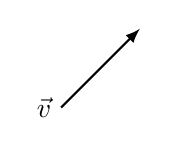
\begin{tikzpicture}
  \draw (0,0) node [left] {$\vec{v}$};
  \draw [-latex, thick] (0,0) -- (1,1);
\end{tikzpicture}

Vector addition takes two vectors and aligns them tail to tip. For example, suppose the following vectors $\vec{a}$, $\vec{b}$ and $\vec{c}$ such that $\vec{a} + \vec{b} = \vec{c}$.

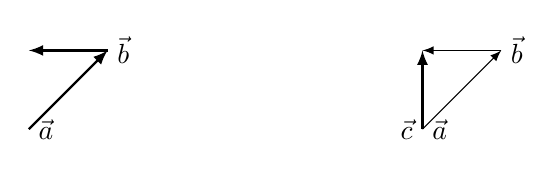
\begin{tikzpicture}
  \draw (0,0) node [right] {$\vec{a}$};
  \draw [-latex, thick] (0,0) -- (1,1);

  \draw (1,1) node [right] {$\vec{b}$};
  \draw [-latex, thick] (1,1) -- (0,1);

  % Two pics

  \draw (5,0) node [right] {$\vec{a}$};
  \draw [-latex] (5,0) -- (6,1);

  \draw (6,1) node [right] {$\vec{b}$};
  \draw [-latex] (6,1) -- (5,1);

  \draw (5,0) node [left] {$\vec{c}$};
  \draw [-latex, thick] (5,0) -- (5,1);

\end{tikzpicture}

\noindent
Vector addition is communative. $\vec{a} + \vec{b} = \vec{b} + \vec{a}$
Vector addition is associativ. $\vec{a} + (\vec{b} + \vec{c}) = (\vec{a} + \vec{b}) + \vec{c}$

\indent
Unit Vectors are vectors of magnitude of 1 that extend in only the x, y, or z direction alone a 3D cartessian system. The vectors are $\hat{i}$, $\hat{j}$ and $\hat{k}$ respectively. Notation for vectors, when expanded, looks like $\vec{A} = (A_x\hat{i} - A_y\hat{j} + A_z\hat{k})$ which could be $=(12\hat{i} - 7\hat{j} + 14\hat{k})$. Vector addition becomes standard addition, and multplying vectors by scalars only needs to be distributed.

\noindent
\Large
Circular Motion\\
\normalsize
\noindent

Angular vectors use radius unit vector ($\hat{r}$) and an inclination unit vector ($\hat{\theta}$). Position around a circle can be determined if given an average velocity and time.\\
Let $T = \frac{2\pi r}{v}$ where $r$ is the radius and $v$ is the velocity.\\
Position: $\vec{r}(t) = r\cos{\frac{2\pi r}{T}}\hat{i} + r\sin{\frac{2\pi r}{T}}\hat{j}$\\
Velocity (derivative of position): $\vec{v}(t) = -r\frac{2\pi}{T}\sin{\frac{2\pi r}{T}}\hat{i} + r\frac{2\pi}{T}\cos{\frac{2\pi r}{T}}\hat{j}$\\
Acceleration (derivative of velocity): $\vec{a}(t) = -r\frac{4\pi^2}{T^2}\cos{\frac{2\pi r}{T}}\hat{i} - r\frac{4\pi^2}{T^2}\sin{\frac{2\pi r}{T}}\hat{j}$\\
Or\\
$\vec{a}_{centrip} = -\frac{v^2}{r}\hat{r}$

\end{document}
